	\makeatletter
	\def\@makechapterhead#1{%
	  \vspace*{50\p@}%
	  {\parindent \z@ \centering\normalfont
	    \ifnum \c@secnumdepth >\m@ne
	      \if@mainmatter
	         \Large\bfseries \@chapapp\space \thechapter
 	        \par\nobreak
	        \vskip 20\p@
	      \fi
	    \fi
	    \interlinepenalty\@M
	     \Large \bfseries #1\par\nobreak
	
	    \vskip 40\p@
	  }}
	\def\@makeschapterhead#1{%
	  \vspace*{50\p@}%
	  {\parindent \z@ \centering 
	    \normalfont
	    \interlinepenalty\@M
	    \Large\bfseries  #1\par\nobreak
	    \vskip 40\p@
	  }}
	\makeatother
	\titlespacing*{\chapter}{0pt}{0pt}{12pt}

\sectionfont{\fontsize{12}}
\titlespacing*{\chapter}{0pt}{0pt}{12pt}
\sectionfont{\fontsize{12}}

\chapter{Database Design}

\section{Introduction}
Database design is the process of producing a detailed data model of a database. This logical data model contains all the needed logical and physical design choices and physical storage parameters needed to generate a design in a Data Definition Language, which can then be used to create a database. A fully attributed data model contains detailed attributes for each entity. 

	\section{System and Database Design}
	
	The database of treasure hunting game system contains three parts, treasure location database, map basic data, and quiz database. Since each treasure location has geographic coordinates, the quiz can automatically appear when the participant is approaching the treasure. The map basic data apply a desktop geographic information system, such as SuperGIS Desktop 2.2 as a platform for creating maps. Then, according to the activity areas, you need to create different maps; for example, the activity held in campus needs to create maps with main buildings, educational buildings, libraries, etc. For the off-campus activities, the maps with main landscapes, roads, rivers, etc are necessary.
	
	The number and levels of quizzes can be arranged by database, and the system can select the quizzes randomly. Therefore, each student might have different quizzes; various relevant quizzes can be designed for the same treasure location. Besides multiple choices, the question type can be fill-in questions with pictures; for example, the system displays the picture of the plants, and the students need to fill in the question.
	
	The set of Treasure Hunting Game adopts SuperGIS Mobile Engine 3, the mobile GIS application SDK (Software Development Kit) as the core object and applies the highly-flexible development mode and complete object controls of SuperGIS Mobile Engine 3 to assist developers in developing intuitive and desired game program.


\begin {table}[H]
\begin{center}
\begin{tabular}{ |l|l|l| }
  \hline
  \multicolumn{3}{|c|}{Question Table} \\
    \hline
  Column Name&Data Type& Length \\
  \hline

qNum&String.&255\\
qQuestion&String.&255\\
qanswer&String.&255\\
qpoints&String.&255\\
qStatus&String.&255\\
qlat&String.&255\\
qlon&String.&255\\
qhint&String.&255\\
  \hline
\end{tabular}
\caption {Question SQL Database} \label{tab:title}
\label{the-label-for-cross-referencing}
\end{center}
\end {table}


\begin {table}[H]
\begin{center}
\begin{tabular}{ |l|l|l| }
  \hline
  \multicolumn{3}{|c|}{ANR Timing} \\
    \hline
  Minimum Response Time &1000.&mili seconds\\
  \hline


Strict Mode & 0 & Disabled \\

  \hline
\end{tabular}
\caption {Application Not Responding Settings} \label{tab:title}
\label{the-label-for-cross-referencing}
\end{center}
\end {table}


\begin {table}[H]
\begin{center}
\begin{tabular}{ |l|l|l| }
  \hline
  \multicolumn{3}{|c|}{Hash Map Mapping} \\
    \hline
  Column Name&Data Type& Length \\
  \hline


id&long.&Integer.Valueof(String) \\
qNum&String.&Integer.Valueof(String)\\
qQuestion&String.&String.Valueof(String)\\
qanswer&String.&String.Valueof(String)\\
qpoints&String.&String.Valueof(String)\\
qStatus&String.&String.Valueof(String)\\
qlat&String.&Double.Valueof(String)\\
qlon&String.&Double.Valueof(String)\\
qhint&String.&String.Valueof(String)\\
  \hline
\end{tabular}
\caption {Hash Map Linked to Simple Adapter} \label{tab:title}
\label{the-label-for-cross-referencing}
\end{center}
\end {table}



\chapter{System Design}

\section{Data Flow Diagram}
A data flow diagram (DFD) is a graphical representation of the “flow” of data through an information system. It differs from the flowchart as it shows the data flow instead of the control flow of the program. A data flow diagram can also be used for the visualization of data processing. \\

\begin{figure}[ht!]
\left
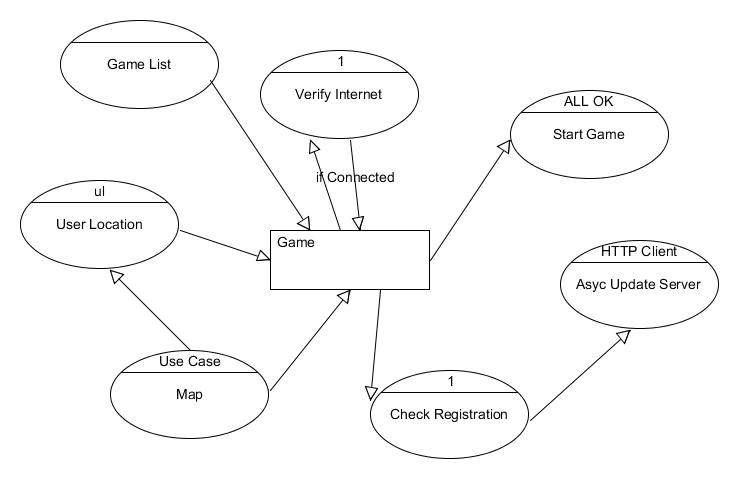
\includegraphics[width=150mm]{images/dfd0}
\caption{Dafa Flow Diagram 0}
\label{overflow}
\end{figure}
\newpage

\begin{figure}[ht!]
\left
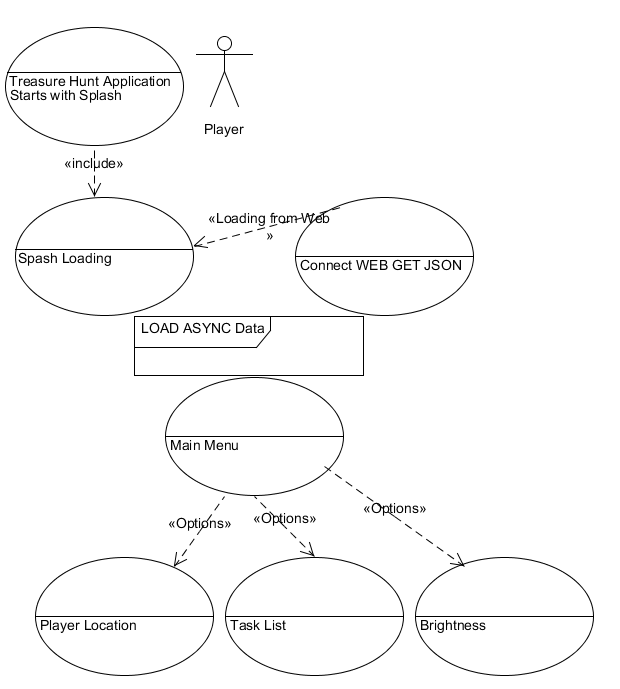
\includegraphics[width=150mm]{dfd0}
\caption{Dafa Flow Diagram 1}
\label{overflow}
\end{figure}
\newpage

\section{Sequence Diagram}
A sequence diagram in UML is a kind of interaction diagram that shows how processes operate with one another and in what order. \\

\begin{figure}[ht!]
\left
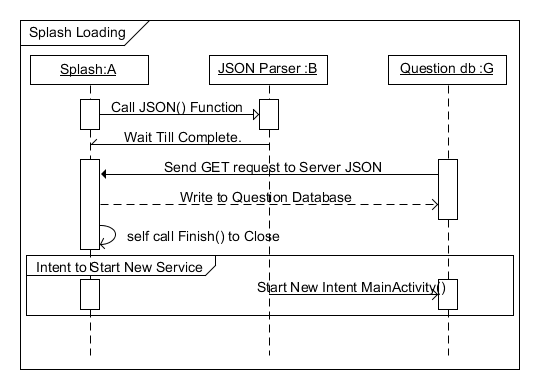
\includegraphics[width=150mm]{splash}
\caption{A simple Splash Screen Loading}
\label{overflow}
\end{figure}
\newpage


\section{Activity Diagram}
Activity diagram are a loosely defined diagram to show workflows of stepwise activities and actions, with support for choice, iteration and concurrency. UML, activity diagrams can be used to describe the business and operational step-by-step workflows of components in a system. 

\begin{figure}[ht!]
\left
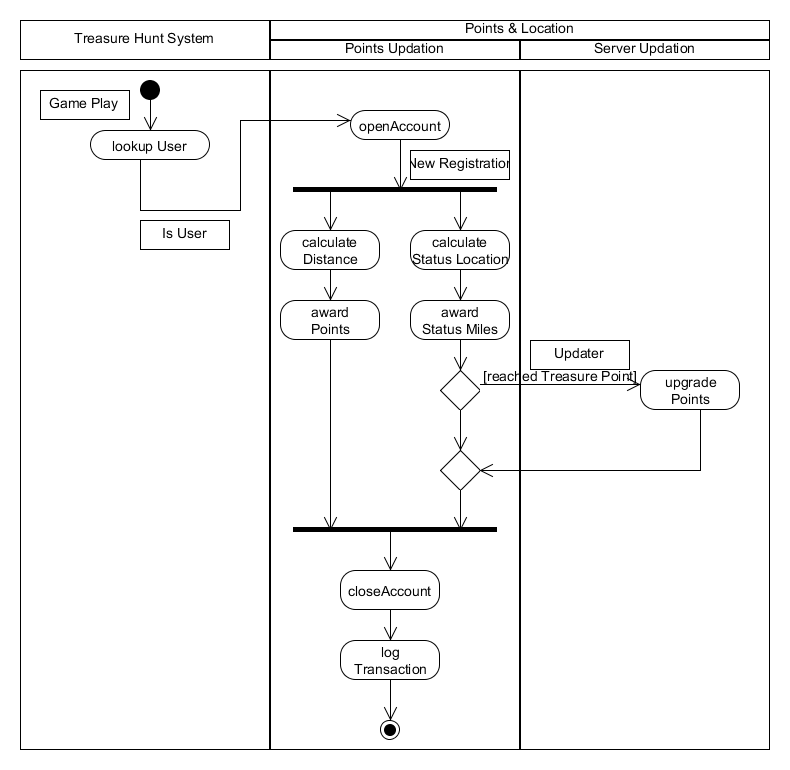
\includegraphics[width=150mm]{images/activityflow}
\caption{Game Checking FLow}
\label{overflow}
\end{figure}

\begin{figure}[ht!]
\left
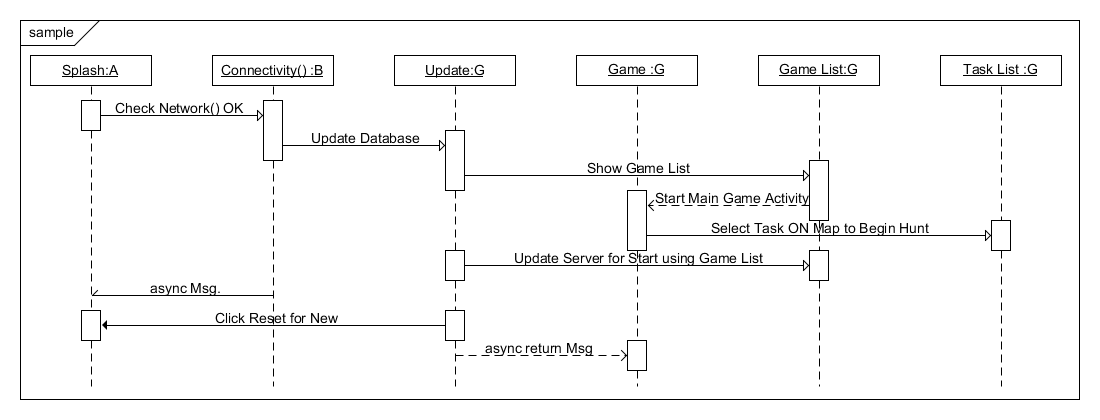
\includegraphics[width=150mm]{reset}
\caption{Game Activity Flow}
\label{overflow}
\end{figure}


\section{Use Case Diagram}
A use case diagram is a graph of actors, a set of use cases enclosed by a system boundary, communication (participation) association between the actors and the use cases, and generalization among the use cases. 

\begin{figure}[ht!]
\left
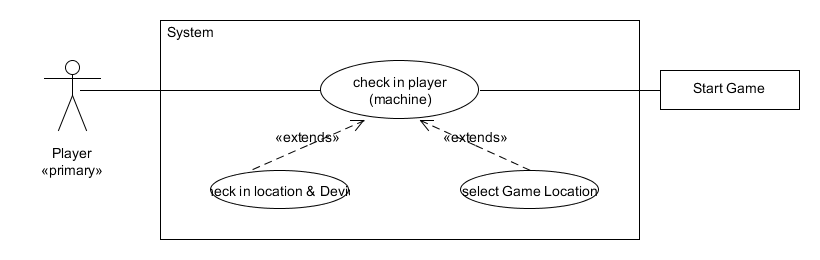
\includegraphics[width=150mm]{images/Usecases}
\caption{Use Case Diagram}
\label{overflow}
\end{figure}



%\section{Class Diagram}
%A class diagram in the UML is a type of static structure diagram that describes the structure of a system by showing the system’s classes, their attributes, and the relationships between the classes. Private visibility hides information from anything outside the class partition. 
%
%\begin{figure}[ht!]
%\centering
%\includegraphics[width=180mm]{cd}
%\caption{A simple caption}
%\label{overflow}
%\end{figure}
%\newpage
%


\newpage
\chapter{Input/Output Design}



\section{Input Design}
The input design is the link between the information system and the user. It comprises the developing specification and procedures for data preparation and those steps are necessary to put transaction data in to a usable form for processing can be achieved by inspecting the computer to read data from a written or printed document or it can occur by having people keying the data directly into the system. The design of input focuses on controlling the amount of input required, controlling the errors, avoiding delay, avoiding extra steps and keeping the process simple. The input is designed in such a way so that it provides security and ease of use with retaining the privacy. Input Design considered the following things:
\begin{itemize}
	
	

	
\item	What data should be given as input?
\item	 How the data should be arranged or coded?
\item	 The dialog to guide the operating personnel in providing input.
\item	Methods for preparing input validations and steps to follow when error occur.
 

\item	Input Design is the process of converting a user-oriented description of the input into a computer-based system. This design is important to avoid errors in the data input process and show the correct direction to the management for getting correct information from the computerized system.
\item It is achieved by creating user-friendly screens for the data entry to handle large volume of data. The goal of designing input is to make data entry easier and to be free from errors. The data entry screen is designed in such a way that all the data manipulates can be performed. It also provides record viewing facilities.
\item	When the data is entered it will check for its validity. Data can be entered with the help of screens. Appropriate messages are provided as when needed so that the user will not be in maize of instant. Thus the objective of input design is to create an input layout that is easy to follow.
\end{itemize}

\section{Output Design}
A quality output is one, which meets the requirements of the end user and presents the information clearly. In any system results of processing are communicated to the users and to other system through outputs. In output design it is determined how the information is to be displaced for immediate need and also the hard copy output. It is the most important and direct source information to the user. Efficient and intelligent output design improves the system’s relationship to help user decision-making.
















